\appendix
\chapter{Lejos Statemachine}
\emph{Lejos Statemachine development toolkit} � una utility per l'ambiente di
sviluppo \emph{Eclipse}, che consente di progettare graficamente una macchina a
stati e implementarla in un brick Lego\textregistered~NXT. Il plugin genera codice \emph{Lejos}, pertanto
consente al programmatore di inserire normale statement Java (comprendendo, chiaramente,
le API di Lejos) all'interno del diagramma a stati.\\
Il manuale ufficiale (in lingua tedesca) del plugin � disponibile al seguente
indirizzo: \url{http://fermat.nordakademie.de/update/Beschreibung.pdf};
l'autore Frank Zimmermann, ne ha prodotto anche un breve riassunto in inglese
che si pu� trovare qui: \url{http://lejos.sourceforge.net/forum/viewtopic.php?t=675}.\\
Una guida completa all'installazione di \emph{Lejos} e di \emph{Lejos
Statemachine development toolkit} � stata scritta in inglese da Juan Antonio
Bre�a Moral e si pu� trovare a questo indirizzo\footnote{I documenti citati in
questo paragrafo sono allegati alla presente relazione.}:
\url{http://www.juanantonio.info/p_articles/archive/2008/LEJOS-NXJ-EBOOK.pdf}
(Capitoli 2.2, 2.3, 3.1).

\section{Ricompilazione del plugin}
La versione ufficiale di \emph{Lejos Statemachine} presente a questo link:
\url{http://fermat.nordakademie.de/update/} e installabile seguendo i
riferimenti forniti in precedenza, � basata su una vecchia versione delle API di
\emph{Lejos}.\\
La release del progetto \emph{Lejos NXJ} pi� recente al momento attuale
(Febbraio 2009) � la \texttt{0.7.0}, se si vuole avere compatibilit� con questa
versione delle API � pertanto necessario ottenere il sorgente (attualmente in
fase di sviluppo) del plugin e compilarlo.

\subsection{Checkout dal repository SVN}
Per prima cosa occorre disporre un ambiente Eclipse provvisto di
\emph{Plug-in Development Environment}, ad esempio la versione \emph{Classic}
disponibile a questo indirizzo: \url{http://www.eclipse.org/downloads/}.\\
Per eseguire il checkout del progetto � necessario installare \emph{Subclipse},
un plugin che integra \emph{Subversion} (Sezione \ref{sec:subversion}) in
\emph{Eclipse}. Per farlo, selezionare il men�
\texttt{Help}$\to$\texttt{Software Updates} e nella sezione \emph{Available Software} selezionare
\texttt{Add Site}.\\
	\begin{figure}
		\begin{center}
			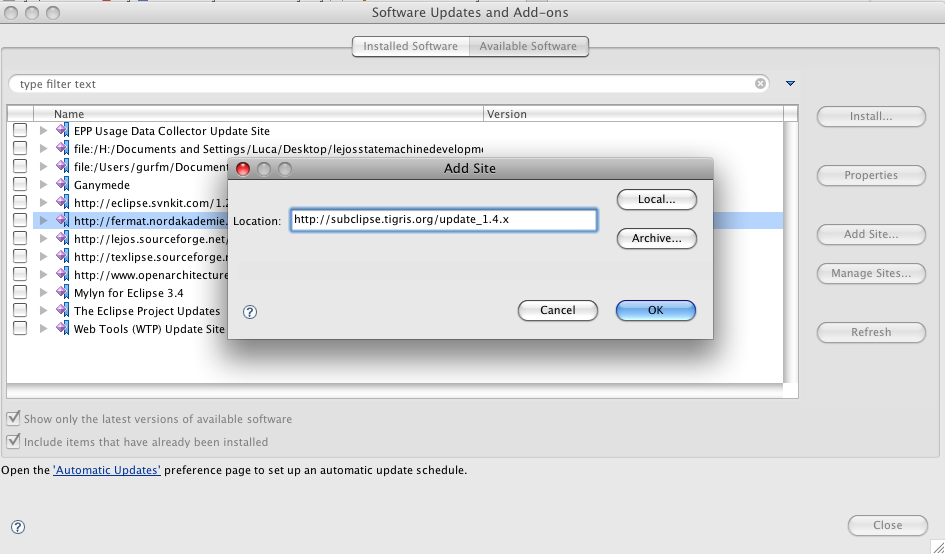
\includegraphics[scale=0.45]{img/howto01.png}
			\caption{Installazione di Subclipse \label{fig:howto01}}
		\end{center}
	\end{figure}
\paragraph{}
Nella finestra di dialogo digitare
\url{http://subclipse.tigris.org/update_1.4.x} e premere \texttt{OK}.\\
Espandere la voce appena aggiunta e selezionare tutti i sotto-elementi (o
almeno quelli evidenziati come \texttt{required} o \texttt{recommended}),
successivamente premere \texttt{Install} e procedere con l'installazione.
	\begin{figure}
		\begin{center}
			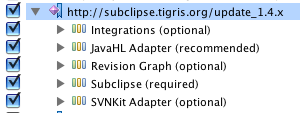
\includegraphics[scale=0.9]{img/howto02.png}
			\caption{Installazione di Subclipse \label{fig:howto02}}
		\end{center}
	\end{figure}
\paragraph{}
Una volta riavviato Eclipse, procedere all'import del progetto in questo modo:
selezionare \texttt{Files}$\to$\texttt{New}$\to$\texttt{Other} e, nella
finestra di dialogo, \texttt{SVN}$\to$\texttt{Checkout projects from SVN},
premere quindi \texttt{Next}.\\
Nella successiva finestra di dialogo selezionare \texttt{Create a new
repository location} e premere \texttt{Next}.
	\begin{figure}
		\begin{center}
			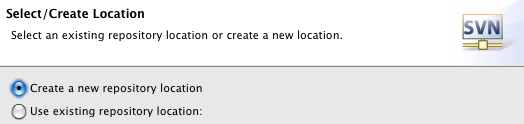
\includegraphics[scale=0.7]{img/howto03.png}
			\caption{Aggiunta del repository\label{fig:howto03}}
		\end{center}
	\end{figure}
\paragraph{}
Digitare l'indirizzo \url{http://svn2.assembla.com/svn/vldt/development/} e
premere ancora \texttt{Next}.\\
	\begin{figure}
		\begin{center}
			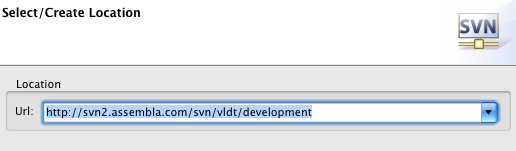
\includegraphics[scale=0.7]{img/howto04.png}
			\caption{Inserimento dell'url del repository SVN \label{fig:howto04}}
		\end{center}
	\end{figure}
Nella finestra successiva selezionare l'intera directory SVN (i.e. tutti i
progetti presenti) e premere \texttt{Finish}.\\
A questo punto il workspace dovrebbe presentarsi come in Figura
\ref{fig:howto05}
	\begin{figure}
		\begin{center}
			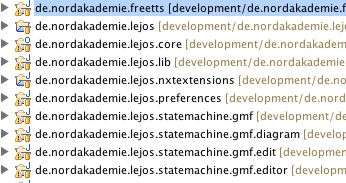
\includegraphics[scale=0.8]{img/howto05.png}
			\caption{Stato finale del workspace\label{fig:howto05}}
		\end{center}
	\end{figure}

\subsection{Modifica del template}
\label{sec:template}
Il codice \texttt{Lejos} generato dal plugin si basa, come gi� evidenziato in
precedenza, sulle API standard, ma anche su una serie di classi facenti parte
del plugin stesso che implementano l'intero meccanismo della macchina a stati,
le transizioni, gli eventi etc\dots\\
Per questo motivo � essenziale che tutti questi helper vengano importati in
testa al programma generato dal parser grafico, infatti il seguente segmento di
codice � sempre presente quando si compila una \emph{Statemachine}:
\begin{lstlisting}
	import de.nordakademie.lejos.statemachine.*;
	import lejos.nxt.*;
	import lejos.navigation.*;
\end{lstlisting}
Questa lista di import � statica e non direttamente accessibile
all'utilizzatore\footnote{A meno di scompattare i files .jar del plugin e
cercare al loro interno il template di traduzione.}, tuttavia a questo livello
� possibile modificarla a piacimento, semplicemente andando ad editare il
template usato per la traduzione in codice \emph{Lejos}. Il file in questione
si trova in \texttt{de.nordakademie.lejos.core/src/template/\\statemachine.xpt},
per il progetto roboCheckers lo si � modificato come segue:
\begin{lstlisting}
[...]
 �EXPAND javaClass(btFlag) FOREACH states.typeSelect(StateMachine)�
 �FILE name+".java"�
    
	import de.nordakademie.lejos.statemachine.*;
	import lejos.nxt.*;
	import lejos.navigation.*;
	import it.polito.Navigation.*;
	import it.polito.util.*;
	import it.polito.Checkers.*;
	import lejos.nxt.addon.ColorSensor;
	import it.polito.BluetoothComm.*;

     public class �name� extends Statemachine{
     
        public �name�(){this(null);} 
[...]
\end{lstlisting}
\newpage
\subsection{Generazione del plugin}
Per esportare il plugin selezionare \texttt{File}$\to$\texttt{Export} e
successivamente \texttt{Plug-in Development}$\to$\texttt{Deployable features},
premere quindi su \texttt{Next}.\\
	\begin{figure}
		\begin{center}
			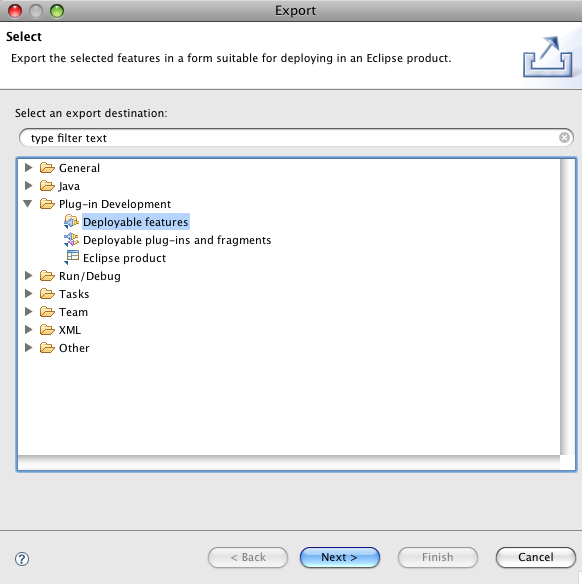
\includegraphics[scale=0.6]{img/howto06.png}
			\caption{Men� Export\label{fig:howto06}}
		\end{center}
	\end{figure}
	\begin{figure}
		\begin{center}
			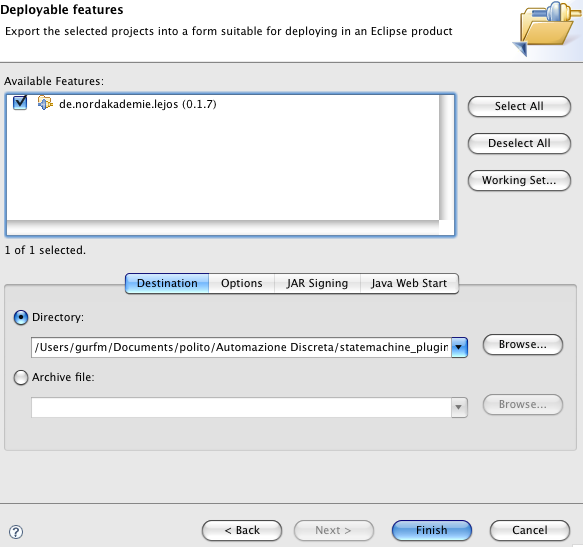
\includegraphics[scale=0.6]{img/howto07.png}
			\caption{Deployable features\label{fig:howto07}}
		\end{center}
	\end{figure}
Nella finestra successiva, selezionare la voce \texttt{de.nordakademie.lejos} e
scegliere una directory di destinazione, prestare attenzione a impostare la
scheda \texttt{Options} come in Figura \ref{fig:howto08}.\\
	\begin{figure}
		\begin{center}
			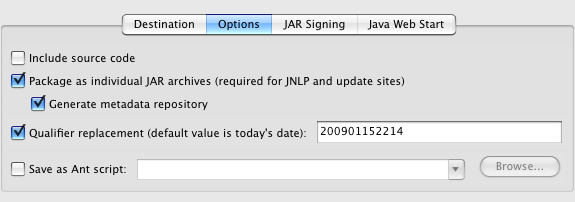
\includegraphics[scale=0.6]{img/howto08.png}
			\caption{Deployable features, options\label{fig:howto08}}
		\end{center}
	\end{figure}
Premere quindi su \texttt{Finish}.\\
\paragraph{}
A questo punto non resta che installare la feature appena generata attraverso
la procedura gi� illustrata per installare i plugin, avendo cura di specificare
la directory locale scelta in precedenza, come repository sorgente nella
finestra di dialogo \texttt{Add Site}.\\
Per evitare conflitti, si consiglia di disinstallare preventivamente qualsiasi
versione del plugin presente in \emph{Eclipse}.

\section{Uso di Lejos Statemachine} 
In questa sezione andiamo ad analizzare gli strumenti forniti dal \emph{Lejos 
Statemachine development toolkit}.\\
Creare un nuovo progetto, mediante \texttt{File}$\to$\texttt{New}$\to$\texttt{Java
Project} e seguire il \emph{wizard}. Il nostro progetto � ora presente nel
\texttt{Package Explorer}: cliccare con il destro su di esso e premere
sulla voce \texttt{leJos NXJ}$\to$\texttt{Convert to leJos NXJ project}.\\
Dal men� contestuale, scegliere \texttt{New}$\to$\texttt{StateMachine Diagram}. Se
tale voce non viene visualizzata, cliccare su \texttt{Other\ldots}: essa � catalogata
sotto la voce \texttt{Lejos StateMachine Diagrams}.
A questo punto selezioniamo il file del diagramma della macchina a stati all'interno 
del nostro progetto facendo doppio click su di esso.
	\begin{figure}
		\begin{center}
			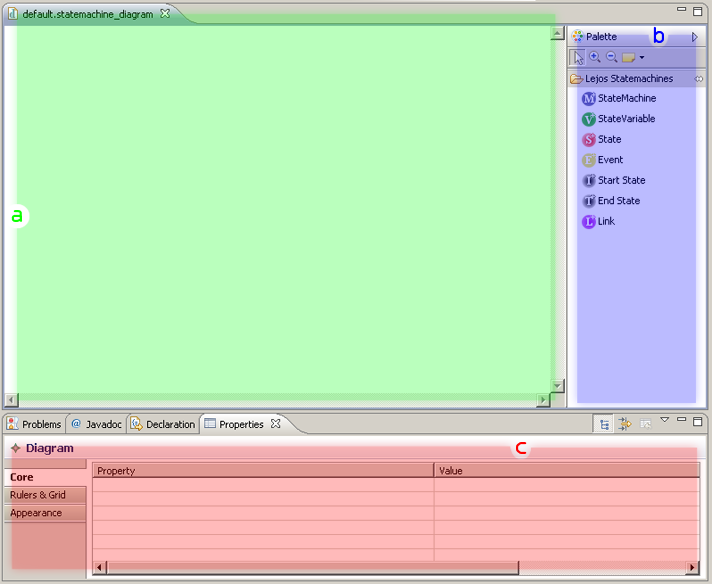
\includegraphics[scale=0.5]{img/lsmgraphicaleditor.png}
			\caption{leJOS StateMachine graphical editor\label{fig:lsmge}}
		\end{center}
	\end{figure}
L'editor grafico � suddiviso in 3 sezioni (Figura \ref{fig:lsmge}):
\begin{itemize}
\item \emph{a}, l'area di lavoro, dove � possibile costruire la \emph{StateMachine}
\item \emph{b}, la casella degli strumenti, dove troviamo tutti gli elementi base
\item \emph{c}, la \texttt{Properties View}, dove ogni elemento pu� essere modificato
sia dal punto di vista comportamentale che estetico (se non viene visualizzata, cliccare 
con il destro sull'area di lavoro e selezionare \texttt{Show Properties View}).
\end{itemize}
Per quanto riguarda gli elementi base di una \emph{StateMachine}, abbiamo:
\begin{itemize}
\item \texttt{StateMachine}, la macchina a stati
\item \texttt{StateVariable}, una variabile di stato
\item \texttt{State}, uno stato
\item \texttt{Event}, un evento
\item \texttt{Start State}, lo stato di partenza (uno o pi� per macchina, ma
ognuno avente una sola transizione uscente)
\item \texttt{End State}, lo stato finale
\item \texttt{Link}, la transizione
\end{itemize}
Le transizioni possono essere di diverso tipo:
\begin{itemize}
\item inserendo un \texttt{Link} tra due \texttt{State}, la transizione avverr� solo
al termine dell'esecuzione del codice del primo (Figura \ref{fig:simple})
\item per far s� che la transizione sia effettuata non appena una certa condizione
viene soddisfatta, � necessario introdurre un \texttt{Event} tra due \texttt{State}
e inserire un blocco di codice in coda alla sezione \emph{do} del primo stato, rendendolo
\emph{interrompibile} (Figura \ref{fig:event})
\end{itemize}
	\begin{figure}
		\begin{center}
			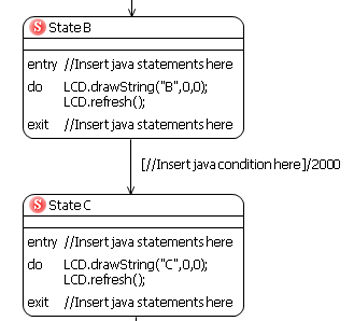
\includegraphics[scale=0.5]{img/simpletransition.png}
			\caption{Transizione semplice\label{fig:simple}}
		\end{center}
	\end{figure}
	\begin{figure}
		\begin{center}
			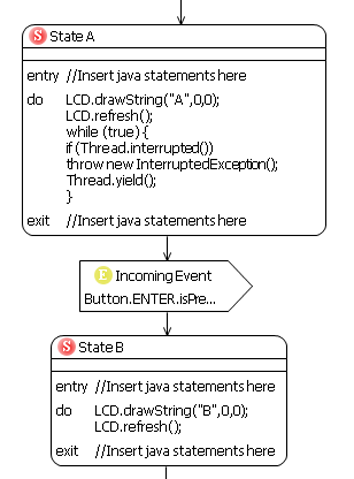
\includegraphics[scale=0.5]{img/eventtransition.png}
			\caption{Transizione ad evento\label{fig:event}}
		\end{center}
	\end{figure}
Il blocco di codice in questione � il seguente:
\begin{lstlisting}
while (true) {
	if (Thread.interrupted())
		throw new InterruptedException();
	Thread.yield();
}
\end{lstlisting}
Procediamo ora nel costruire una macchina a stati d'esempio.\\
Selezionare l'elemento \texttt{StateMachine} dalla casella degli strumenti e tracciare
un rettangolo nell'area di lavoro.
Attraverso la \texttt{Properties View} � possibile modificarne il nome.
Introduciamo all'interno della \texttt{StateMachine} uno \texttt{Start State} e gli
\texttt{State} necessari per realizzare il flusso del processo richiesto.
I \texttt{Link} possono essere creati selezionando \texttt{Link} nella casella degli strumenti
ed effettuando un \emph{drag and drop} dal primo al secondo elemento da collegare.
E' possibile assegnare delle condizioni alle transizioni, ma la copertura deve essere completa:
uno stato che ha eseguito le proprie istruzioni deve avere una transizione uscente \emph{valida},
altrimenti la macchina a stati salter� allo stato \texttt{End State}.
Sono disponibili due \emph{ScreenCast}: 
\begin{itemize}
\item StateMachine semplice
\url{http://www.screentoaster.com/watch/stUk1dSkVLRlxeRF9fU11Z}
\item StateMachine con due processi
\url{http://www.screentoaster.com/watch/stUk1dSkVLRlxeRF5aWV9c}
\end{itemize}
